\section{Data integration}

\begin{frame}{Data Integration}
	\begin{itemize}
		\item \textbf{Data integration:}
		      \begin{itemize}
			      \item Combine data from multiple sources into a coherent store.
		      \end{itemize}
		\item \textbf{Schema integration:}
		      \begin{itemize}
			      \item E.g. \texttt{A.cust-id} $\equiv$ \texttt{B.cust-\#}.
			      \item Integrate metadata from different sources.
		      \end{itemize}
		\item \textbf{Entity-identification problem:}
		      \begin{itemize}
			      \item Identify the same real-world entities from multiple data
			            sources.
			      \item E.g. Bill Clinton = William Clinton.
		      \end{itemize}
		\item \textbf{Detecting and resolving {\color{airforceblue}data-value
					      conflicts}:}
		      \begin{itemize}
			      \item For the same real world entity, attribute values from
			            different sources are different.
			      \item Possible reasons:
			            \begin{itemize}
				            \item Different representations (coding).
				            \item Different scales, e.g. metric vs. British units.
			            \end{itemize}
		      \end{itemize}
	\end{itemize}
\end{frame}

\begin{frame}{Handling Redundancy in Data Integration}
	\begin{itemize}
		\item \textbf{Redundant data often occur when integrating multiple
			      databases.}
		      \begin{itemize}
			      \item \textbf{Object (entity) identification:} \\
			            The same attribute or object may have different names in different
			            databases.
			      \item \textbf{Derivable data:}\\
			            One attribute may be a "derived" attribute in another table. E.g.
			            annual revenue.
		      \end{itemize}
		\item \textbf{Redundant attributes:}
		      \begin{itemize}
			      \item Can be detected by \textbf{\color{airforceblue}correlation
				            analysis} and \textbf{\color{airforceblue}covariance analysis}.
		      \end{itemize}
		\item \textbf{Careful integration of the data from multiple sources:}
		      \begin{itemize}
			      \item Helps to reduce/avoid redundancies and inconsistencies and
			            improve mining speed and quality.
		      \end{itemize}
	\end{itemize}
\end{frame}

\begin{frame}{Correlation Analysis for Nominal Data (I)}
	\begin{itemize}
		\item \textbf{Example:}

		      We want to determine if the interests "Reads Books" and
		      "Plays Chess" in the following table correlate with each other:

		      \vspace{5mm}

		      \begin{center}
			      \begin{tabular}{|l|c|c|}
				      \hline
				      ID       & Reads Books & Plays Chess
				      \\\hline
				      1        & Y           & Y
				      \\\hline
				      2        & Y           & Y
				      \\\hline
				      3        & Y           & N
				      \\\hline
				      $\ldots$ & $\ldots$    & $\ldots$
				      \\\hline
				      1499     & N           & Y
				      \\\hline
				      1500     & N           & N
				      \\\hline
			      \end{tabular}
		      \end{center}
	\end{itemize}
\end{frame}

\begin{frame}{Correlation Analysis for Nominal Data (II)}
	\begin{columns}
		\begin{column}{0.5\textwidth}
			\begin{itemize}
				\item \textbf{General starting point:}
				      \begin{itemize}
					      \item \textbf{The attributes A and B to be analyzed:}
					            \begin{itemize}
						            \item $A$ has $n$ distinct values: $A :=
							                  \{a_1, a_2, \ldots, a_n\}$, where $n \in
							                  \mathbb{N}_{>1}$.
						            \item $B$ has $m$ distinct values: $B :=
							                  \{b_1, b_2, \ldots, b_m\}$ , where $m \in
							                  \mathbb{N}_{>1}$.
					            \end{itemize}
					      \item \textbf{The set X of all distinct combinations:}
					            \begin{itemize}
						            \item $X$ is defined as follows: \\
						                  $X := \{(a, b) \; \vert \; a \in A \;
							                  \text{and} \; b \in B\}$.
					            \end{itemize}
					      \item \textbf{The multi set Y of all tuples:}
					            \begin{itemize}
						            \item The multiset $Y$ over the set $X$
						                  is a mapping of $X$ to the set of natural
						                  numbers $\mathbb{N}_{0}$.
						                  The number $Y(x), x \in X$ tells
						                  how often $x$ is contained in the multiset
						                  $Y$.
					            \end{itemize}
				      \end{itemize}
			\end{itemize}
		\end{column}
		\begin{column}{0.5\textwidth}
			\begin{itemize}
				\item \textbf{Starting point in the example:}
				      \begin{itemize}
					      \item \textbf{The attributes A and B to be analyzed:}
					            \begin{itemize}
						            \item $A$ ("Reads Books") has $2$ distinct
						                  values: \\
						                  $A := \{Y, N\}$
						            \item $B$ ("Plays Chess") has $2$ distinct values: \\
						                  $B := \{Y, N\}$
					            \end{itemize}
					      \item \textbf{The set X of all distinct combinations:}
					            \begin{itemize}
						            \item $X$ contains $4$ distinct combinations: \\
						                  $X := \{(Y, Y), (Y, N), (N, Y), (N, N)\}$.
					            \end{itemize}
					      \item \textbf{The multi set Y of all tuples:}
					            \begin{itemize}
						            \item $Y$ contains $1500$ tuples: \\
						                  $Y := \{(Y, Y), (Y, Y), \ldots, (N, N)\}$.
					            \end{itemize}
				      \end{itemize}
			\end{itemize}
		\end{column}
	\end{columns}
\end{frame}

\begin{frame}{Correlation Analysis for Nominal Data (III)}
	\begin{itemize}
		\item \textbf{Actual quantity in $Y$:}
		      \begin{align*}
			      c_{ij} = \#\{(a,b) \in Y \; \vert \; a = a_i, b= b_i\}
			      = Y((a_i, b_j))
		      \end{align*}
		\item \textbf{Expected quantity (value of $c_{ij}$) in case of
			      independence, i.\,e.\ no correlation:}
		      \begin{align*}
			      e_{ij} = \frac{\sum_{k=1}^{m} c_{ik}}{\#Y} \cdot
			      \frac{\sum_{l=1}^{n}c_{lj}}{\#Y} \cdot \#Y
			      = \frac{\sum_{k=1}^{m} c_{ik} \cdot \sum_{l=1}^{n}c_{lj}}{\#Y}
		      \end{align*}
	\end{itemize}

	\begin{block}{Please note that:}
		\begin{itemize}
			\item The sum of all $c_{ij}$ over an attribute $a_i$ (or $b_j$) is
			      identical to the sum of all $e_{ij}$ over $a_i$ (or $b_j$):
			      \vspace{-2mm}
			      \begin{align*}
				      \sum_{k=1}^{m} e_{ik} = \sum_{k=1}^{m} c_{ik} \textit{ and }
				      \sum_{l=1}^{n} e_{lj} = \sum_{l=1}^{n} c_{lj}
			      \end{align*}
		\end{itemize}
	\end{block}
\end{frame}


\begin{frame}{Correlation Analysis for Nominal Data (IV)}
	\begin{itemize}
		\item \textbf{The values $c_{ij}$ and $e_{ij}$ are often presented in a
			      \color{airforceblue} contingency table:} \\
		      \begin{center}
			      \vspace{1mm}
			      \begin{tabular}{|l|c|c|c|c|}
				      \hline
				               & $a_1$                             & $\ldots$ & $a_n$             &
				      \\\hline
				      $b_1$    & $c_{11} (e_{11})$                 & $\ldots$ & $c_{n1} (e_{n1})$ &
				      $\sum_{i=1}^n e_{i1}$
				      \\\hline
				      $\ldots$ & $\ldots$                          & $\ldots$ & $\ldots$          & $\ldots$
				      \\\hline
				      $b_m$    & $c_{1m} (e_{1m})$                 & $\ldots$ & $c_{nm} (e_{nm})$ &
				      $\sum_{i=1}^n e_{im}$
				      \\\hline
				               & $\sum_{j=1}^m e_{1j}$             & $\ldots$ & $\sum_{j=1}^m
				      e_{nj}$  & $\sum_{i=1}^n\sum_{j=1}^m e_{ij}$
				      \\\hline
			      \end{tabular}
			      \vspace{2mm}
		      \end{center}
		\item \textbf{In our example it would look like this:} \\
		      \begin{center}
			      \vspace{1mm}
			      \begin{tabular}{|l|c|c|c|}
				      \hline
				                         & Plays chess & Doesn't play chess & Sum (row)
				      \\\hline
				      Reads books        & $250 (90)$  & $200 (360)$        & $450$
				      \\\hline
				      Doesn't read books & $50 (210)$  & $1000 (840)$       &
				      $1050$
				      \\\hline
				      Sum (column)       & $300$       & $1200$             & $1500$
				      \\\hline
			      \end{tabular}
		      \end{center}
	\end{itemize}
\end{frame}

\begin{frame}{Correlation Analysis for Nominal Data (V)}
	\begin{itemize}
		\item \textbf{To determine the correlation the
				      {\color{airforceblue}$\chi^2$-test} (Chi-squared test) is
			      applied:}
		      \begin{align*}
			      \chi^2 = \sum_{i=1}^{n}\sum_{j=1}^{m}
			      \frac{(c_{ij}-e_{ij})^2}{e_{ij}}.
		      \end{align*}
		      \begin{block}{Properties of the $\chi^2$-test}
			      \begin{itemize}
				      \item No correlation (i.e. independence of attributes) yields
				            $\chi^2$
				            value of zero.
				      \item The larger the $\chi^2$ value, the more likely the
				            variables are
				            related.
				      \item The cells that contribute the most to the $\chi^2$ value
				            are those whose actual count is very different from the
				            expected count
				            $e_{ij}$.
			      \end{itemize}
		      \end{block}
	\end{itemize}
\end{frame}

\begin{frame}{Correlation Analysis for Nominal Data (VI)}
	\begin{itemize}
		\item \textbf{Calculation of $\chi^2$ in our example:}
		      \begin{align*}
			      \chi^2 = \frac{(250-90)^2}{90} + \frac{(50-210)^2}{210} +
			      \frac{(200-360)^2}{360} + \frac{(1000-840)^2}{840} = 507.93.
		      \end{align*}
		\item \textbf{It shows that "Reads Books" and "Plays Chess" are
			      correlated (in our example)}
		      \vspace{5mm}
		      \begin{alertblock}{Important: Correlation does not imply causality!}
			      \begin{itemize}
				      \item E.g. $\#$ of hospitals and $\#$ of car-thefts in a city
				            are correlated.
				      \item Both are causally linked to the third variable:
				            population.
			      \end{itemize}
		      \end{alertblock}
	\end{itemize}
\end{frame}

\begin{frame}{Correlation Analysis of Numerical Data (I)}
	\begin{itemize}
		\item \textbf{Numerical correlation can be determined with
				      {\color{airforceblue}Pearson's product-moment coefficient}:}
		      \begin{align*}
			      \text{Cor}(A, B) = \frac{\sum_{i=1}^{n}
				      (a_i-\mu_{A})(b_i-\mu_{B})}{n\cdot\sigma_{A}\sigma_{B}} =
			      \frac{\sum_{i=1}^{n} a_i b_i -n\cdot\mu_{A}\mu_{B}}{n\cdot
				      \sigma_{A}\sigma_{B}}.
		      \end{align*}
		      where $n$ is the number of tuples, $a_i$ and $b_i$ are the
		      respective values of $A$ and $B$ in tuple $i$,
		      $\mu_A$ and $\mu_B$ are the respective mean values of $A$ and $B$,
		      $\sigma_{A}$ and $\sigma_{B}$B are the respective standard
		      deviations of $A$ and $B$
		      \begin{block}{Properties of Pearson's product-moment coefficient}
			      \begin{itemize}
				      \item If $\text{Cor}(A, B) > 0$: $A$ and $B$ are positively
				            correlated.
				      \item If $\text{Cor}(A, B) = 0$: $A$ and $B$ are independent.
				      \item If $\text{Cor}(A, B) < 0$: $A$ and $B$ are negatively
				            correlated.
			      \end{itemize}
		      \end{block}
	\end{itemize}
\end{frame}

\begin{frame}{Correlation Analysis of Numerical Data (II)}
	\begin{itemize}
		\item \textbf{It is also possible to visually detect numerical
			      correlation:}

		      \vspace{2mm}

		      \begin{figure}[H]
			      \centering
			      \begin{minipage}{0.28\textwidth}
				      \centering
				      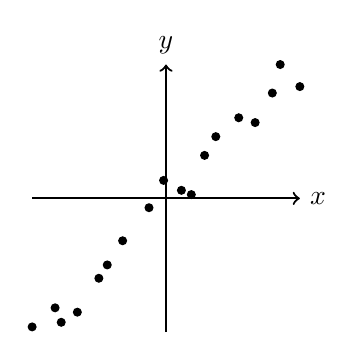
\begin{tikzpicture}
					      \draw[->, thick] (-1.7,0)--(1.7,0) node[right]{$x$};
					      \draw[->, thick] (0,-1.7)--(0,1.7) node[above]{$y$};
					      \foreach \x in {-1.7,-1.5,...,1.7}{
							      \pgfmathsetmacro\xcoord{\x+rand/10}
							      \pgfmathsetmacro\ycoord{\x+rand/2}
							      \pgfmathsetmacro\xcoord{\xcoord < -1.7 ? -1.7 :
								      \xcoord}
							      \pgfmathsetmacro\xcoord{\xcoord > 1.7 ? 1.7 :
								      \xcoord}
							      \pgfmathsetmacro\ycoord{\ycoord < -1.7 ? -1.7 :
								      \ycoord}
							      \pgfmathsetmacro\ycoord{\ycoord > 1.7 ? 1.7 :
								      \ycoord}
							      \node[circle,draw,fill=black,scale=0.3] at
							      (\xcoord,\ycoord) {};
						      }
				      \end{tikzpicture}
				      \caption{a) Positive correlation.}
			      \end{minipage}\hfill
			      \begin{minipage}{0.32\textwidth}
				      \centering
				      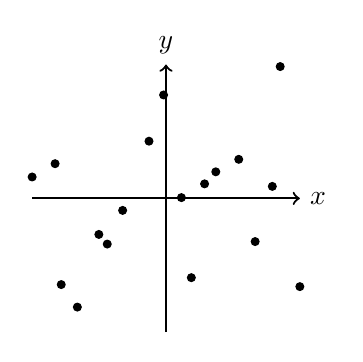
\begin{tikzpicture}
					      \draw[->, thick] (-1.7,0)--(1.7,0) node[right]{$x$};
					      \draw[->, thick] (0,-1.7)--(0,1.7) node[above]{$y$};
					      \foreach \x in {-1.7,-1.5,...,1.7}{
							      \pgfmathsetmacro\xcoord{\x+rand/10}
							      \pgfmathsetmacro\ycoord{rand*2}
							      \pgfmathsetmacro\xcoord{\xcoord < -1.7 ? -1.7 :
								      \xcoord}
							      \pgfmathsetmacro\xcoord{\xcoord > 1.7 ? 1.7 :
								      \xcoord}
							      \pgfmathsetmacro\ycoord{\ycoord < -1.7 ? -1.7 :
								      \ycoord}
							      \pgfmathsetmacro\ycoord{\ycoord > 1.7 ? 1.7 :
								      \ycoord}
							      \node[circle,draw,fill=black,scale=0.3] at
							      (\xcoord,\ycoord) {};
						      }
				      \end{tikzpicture}
				      \caption{b) Uncorrelated/no correlation.}
			      \end{minipage}\hfill
			      \begin{minipage}{0.32\textwidth}
				      \centering
				      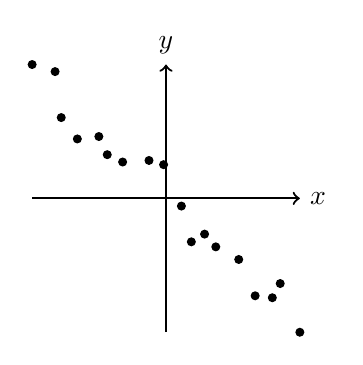
\begin{tikzpicture}
					      \draw[->, thick] (-1.7,0)--(1.7,0) node[right]{$x$};
					      \draw[->, thick] (0,-1.7)--(0,1.7) node[above]{$y$};
					      \foreach \x in {-1.7,-1.5,...,1.7}{
							      \pgfmathsetmacro\xcoord{\x+rand/10}
							      \pgfmathsetmacro\ycoord{-\x+rand/2}
							      \pgfmathsetmacro\xcoord{\xcoord < -1.7 ? -1.7 :
								      \xcoord}
							      \pgfmathsetmacro\xcoord{\xcoord > 1.7 ? 1.7 :
								      \xcoord}
							      \pgfmathsetmacro\ycoord{\ycoord < -1.7 ? -1.7 :
								      \ycoord}
							      \pgfmathsetmacro\ycoord{\ycoord > 1.7 ? 1.7 :
								      \ycoord}
							      \node[circle,draw,fill=black,scale=0.3] at
							      (\xcoord,\ycoord) {};
						      }
				      \end{tikzpicture}
				      \caption{c) Negative correlation.}
			      \end{minipage}\hfill
		      \end{figure}
	\end{itemize}
\end{frame}

\begin{frame}{Covariance of Numerical Data (I)}
	\begin{itemize}
		\item \textbf{\color{airforceblue}Covariance} \textbf{is similar to
			      correlation:}
		      \begin{align*}
			      \text{Cov}(A, B) =
			      \frac{\sum_{i=1}^{n}(a_i-\mu_{A})(b_i-\mu_{B})}{n} =
			      \frac{\sum_{i=1}^{n}a_ib_i}{n}-\mu_{A}\mu_{B}
		      \end{align*}
		\item \textbf{It is possible to compute the correlation based on the
			      covariance:}
		      \begin{align*}
			      \text{Cor}(A, B) = \frac{\text{Cov}(A,
				      B)}{\sigma_{A}\sigma_{B}}
		      \end{align*}
	\end{itemize}
	\begin{block}{Properties of the covariance}
		\begin{itemize}
			\item If $\text{Cov}(A, B) > 0$: $A$ and $B$ tend to be either both
			      larger or both smaller than their expected values.
			\item If $\text{Cov}(A, B) < 0$: If $A$ is larger than its expected
			      value, $B$ is likely to be smaller than its expected value and vice
			      versa.
		\end{itemize}
	\end{block}
\end{frame}

\begin{frame}{Covariance of Numerical Data (II)}
	\begin{itemize}
		\item \textbf{Example:}
		      \begin{itemize}
			      \item We examine a table containing the history of two
			            stock prices:

			            \begin{center}
				            \begin{tabular}{|l|c|c|}
					            \hline
					            Date  & Stock 1 & Stock 2
					            \\\hline
					            21.06 & 2       & 5
					            \\\hline
					            22.06 & 3       & 8
					            \\\hline
					            23.06 & 5       & 10
					            \\\hline
					            24.06 & 4       & 11
					            \\\hline
					            25.06 & 6       & 14
					            \\\hline
				            \end{tabular}
			            \end{center}

			            \vspace{1mm}

			      \item If the stocks are affected by the same industry trends,
			            will their prices rise or fall together?
			            \begin{align*}
				            \text{Cov}(A, B) & = \frac{2\cdot5 + 3\cdot 8 + 5
					            \cdot
					            10 + 4 \cdot 11 + 6 \cdot 14}{5} - 4\cdot 9.6 = 4.
			            \end{align*}
			      \item Thus, $A$ and $B$ rise together since $\text{Cov}(A, B) >
				            0$.
		      \end{itemize}
	\end{itemize}
\end{frame}
